\chapter{Design di dettaglio}\label{ch:design-di-dettaglio}
In seguito alla realizzazione del design architetturale di massima sono state effettuate scelte rilevanti
ai fini della progettazione di alcune parti del sistema.

\section{Lista di componenti}\label{sec:lista-di-componenti}
Come emerge dal design architetturale, i sistemi e le viste indicano, a livello del proprio tipo, su quali
componenti andranno ad operare.
Per indicare queste liste di tipi si è scelto di utilizzare le \texttt{CList} (abbreviazione di \textit{Components List})
che sono essenzialmente liste di elementi eterogenei che preservano informazioni sui tipi dei propri elementi in maniera
simile alle tuple.

L’idea alla base di questa soluzione è ispirata dalle \textit{Heterogeneous List} della libreria
Shapeless~\cite{shapeless}.

\section{Container di componenti}\label{sec:container-di-componenti}
Come è possibile osservare in Figura~\ref{fig:world-detail}, dal design architetturale emerge come
non siano le entità stesse a possedere i componenti che vengono loro assegnati.
Infatti, la gestione dei componenti è demandata a un container di componenti;
questo permette di aggiungere o rimuovere coppie entità-componente oppure di ottenere tutte le entità con uno specifico
tipo di componente.
In questo modo è possibile introdurre in maniera semplice ottimizzazioni nella gestione dei
componenti per rendere la loro iterazione (fondamentale per i sistemi) quanto più veloce possibile.

Grazie a questa scelta è stato piuttosto semplice modificare l'implementazione del container per attuare ottimizzazioni
necessarie a rispettare il requisito non funzionale~\ref{itm:nf1}.
\begin{figure}[H]
    \centering
    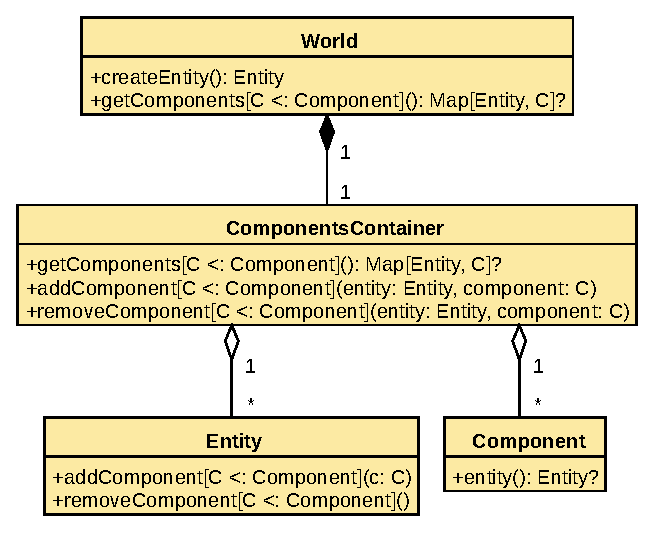
\includegraphics[width=\textwidth]{./img/WorldDetail}
    \caption{Design di dettaglio di \texttt{World} e \texttt{Entities}.}
    \label{fig:world-detail}
\end{figure}

\section{Builder dei sistemi}\label{sec:builder-dei-sistemi}
Si è scelto di realizzare il pattern Builder per permettere una creazione di sistemi quanto più semplice possibile.
Come mostrato nel diagramma riportato in Figura~\ref{fig:system-builder} il builder dispone di diversi
metodi per specificare l'implementazione di alcuni dei metodi del sistema che verrà costruito.
Per completare la costruzione tramite il builder e ottenere il nuovo sistema bisogna specificare
(tramite il metodo \texttt{withUpdate}) l'implementazione del suo metodo \texttt{update}.

\begin{figure}[H]
    \centering
    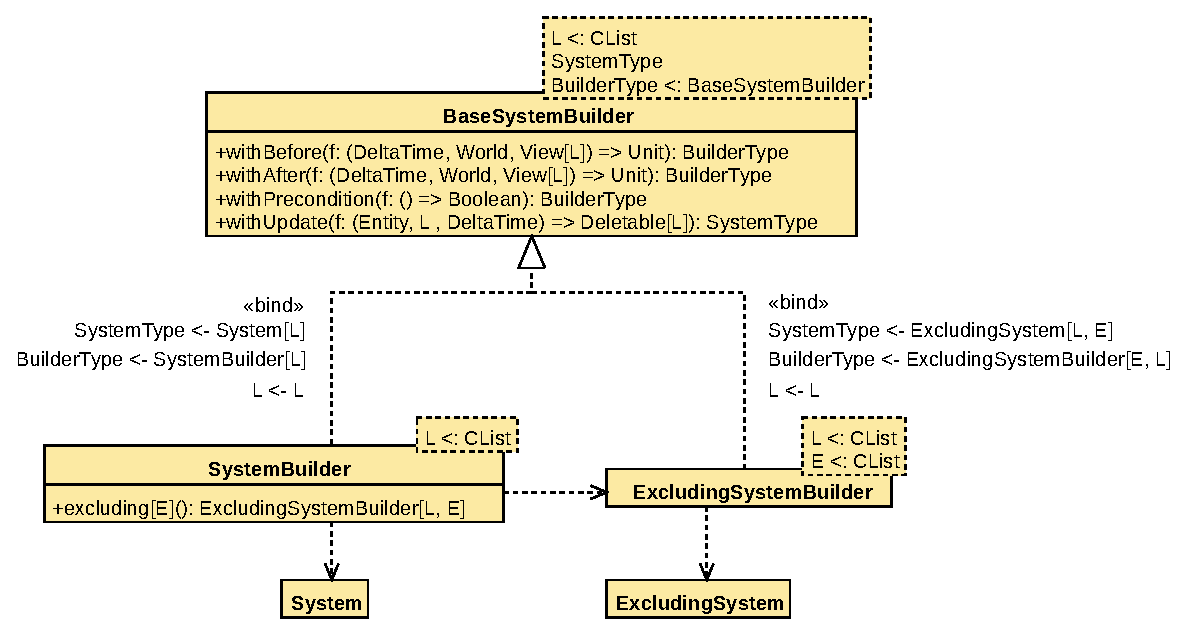
\includegraphics[width=\textwidth]{./img/SystemBuilder}
    \caption{Design di dettaglio del \texttt{SystemBuilder}.}
    \label{fig:system-builder}
\end{figure}
